\newcommand{\DoNotLoadEpstopdf}{}
\documentclass[11pt]{article}
\ifdefined\pdfinfoomitdate\pdfinfoomitdate=1\fi
\ifdefined\pdftrailerid\pdftrailerid{}\fi
\ifdefined\pdfsuppressptexinfo\pdfsuppressptexinfo=15\fi
\input{glyphtounicode}
\pdfglyphtounicode{parenleftbig}{0028}
\pdfglyphtounicode{parenrightbig}{0029}
\pdfglyphtounicode{parenleftBigg}{0028}
\pdfglyphtounicode{parenrightBigg}{0029}
\pdfglyphtounicode{braceleftBigg}{007B}
\pdfglyphtounicode{summationtext}{2211}
\pdfglyphtounicode{summationdisplay}{2211}
\pdfglyphtounicode{uniontext}{22C3}
\pdfglyphtounicode{logicalordisplay}{22C1}
\pdfglyphtounicode{hatwide}{0302}
\pdfgentounicode=1

\usepackage[T1]{fontenc}
\usepackage{lmodern}
\usepackage{amsmath,amssymb,amsthm,mathtools}
\usepackage[margin=1.08in]{geometry}
\usepackage{microtype}
\usepackage{enumitem}
\usepackage{tikz}
\usetikzlibrary{arrows.meta}
\usepackage[colorlinks=true,linkcolor=blue,citecolor=blue,urlcolor=blue]{hyperref}
\hypersetup{pdftitle={Rigidity of the Turing degrees},pdfauthor={OpenAI}}
\setlength{\emergencystretch}{1.5em}
\setlist[enumerate]{leftmargin=*,itemsep=3pt,topsep=4pt}
\setlist[itemize]{leftmargin=*,itemsep=3pt,topsep=4pt}
\numberwithin{equation}{section}
\newtheorem{theorem}{Theorem}[section]
\newtheorem{proposition}[theorem]{Proposition}
\newtheorem{lemma}[theorem]{Lemma}
\newtheorem{corollary}[theorem]{Corollary}
\theoremstyle{remark}
\newtheorem{remark}[theorem]{Remark}
\newcommand{\N}{\mathbb N}
\newcommand{\Q}{\mathbb Q}
\newcommand{\R}{\mathbb R}
\newcommand{\DT}{\mathcal D_T}
\newcommand{\leT}{\le_T}
\newcommand{\equivT}{\equiv_T}
\newcommand{\degT}[1]{[#1]_T}
\DeclareMathOperator{\Aut}{Aut}
\title{Rigidity of the Turing degrees}
\author{OpenAI}
\date{September 24, 2026}
\begin{document}
\maketitle
\begin{abstract}
We prove that every order automorphism of the full partial order of
Turing degrees is the identity, resolving the rigidity conjecture for
the Turing degrees positively.
\end{abstract}
\section{Introduction}\label{sec:introduction}

Turing reducibility compares the information available from sets of
integers: $A\leT B$ means that an oracle Turing machine with oracle $B$
computes the characteristic function of $A$. Mutual reducibility
defines Turing equivalence, and its equivalence classes form the
partial order $(\DT,\leT)$ of Turing degrees. The underlying notion
of relative computation goes back to Turing's oracle machines
\cite[Section~4]{Turing1939}; see \cite{Soare1987} for standard
degree-theoretic background. The automorphism problem asks how much
of this information the abstract ordering retains.

The rigidity conjecture for the Turing degrees asks whether every
automorphism of this ordering fixes every degree.
An automorphism here is any bijection
$\pi:\DT\to\DT$ satisfying
\[
\mathbf a\leT\mathbf b
\quad\Longleftrightarrow\quad
\pi(\mathbf a)\leT\pi(\mathbf b).
\]
We work in ZFC and impose no definability or regularity hypothesis
on $\pi$.

\begin{theorem}\label{thm:rigidity}
Every order automorphism of the full Turing-degree structure is
the identity:
\[
\forall\pi\in\Aut(\DT,\leT)\ \forall\mathbf a\in\DT
\qquad \pi(\mathbf a)=\mathbf a.
\]
\end{theorem}

\paragraph{Prior work and the remaining problem.}
The Turing jump sends a degree $\mathbf a$ to the degree
$\mathbf a'$ of the halting problem relative to an oracle of
degree $\mathbf a$. Jockusch and Solovay proved that every
jump-preserving order automorphism fixes all degrees above
$\mathbf0^{(4)}$, the fourth jump of the computable degree
\cite{JockuschSolovay1977}. Using Slaman and Woodin's definability
of the double jump, Shore and Slaman proved that the jump is
definable from the ordering
\cite{ShoreSlaman1999}, so every order automorphism preserves it.
Shore later gave direct degree-theoretic definitions of the jump
\cite{Shore2007}.

A cone consists of all degrees above a fixed degree. Nerode and
Shore proved that every automorphism fixes some cone, whose base
may depend on the automorphism \cite{NerodeShore1980}; see also
\cite[Theorem~3.2, author's version]{SlamanGlobal}.
Slaman and Woodin obtained a fixed cone common to all
automorphisms: every automorphism fixes all degrees above
$\mathbf0''$, the second jump of the computable degree.
Their analysis also shows that the automorphism group is
countable and that each automorphism has an arithmetic
representation on sets of integers
\cite{SlamanWoodin2005,SlamanGlobal}.
These results show that the order determines substantial
computability-theoretic structure. They leave the rigidity
problem at degrees outside the known fixed cone.

The representation theorem is the external input to our proof.
In its all-input form, it assigns to every arbitrary degree
automorphism a single arithmetic, hence Borel, function on sets of
integers that induces that automorphism on degrees
\cite[Theorem~6.3.1(2)]{SlamanWoodin2005}. The cited source is the
2005 unpublished manuscript; the result also appears in Slaman's
account \cite{SlamanGlobal}. This theorem supplies the regularity
needed for a category argument while retaining the unrestricted
scope of Theorem~\ref{thm:rigidity}.

\paragraph{A consequence for definability.}
Theorem~\ref{thm:rigidity} also settles the biinterpretability
conjecture of Slaman and Woodin. Full second-order arithmetic is
the two-sorted structure of natural numbers and all subsets of
natural numbers, with arithmetic and membership. Slaman and Woodin
interpret this structure using finite tuples of Turing degrees.
In their formulation, biinterpretability asks whether the relation
matching such a code for a set $X\subseteq\N$ with its degree
$\degT X$ is first-order definable in the degree ordering without
parameters \cite[Definition~7.5.1]{SlamanWoodin2005}.
They prove that this is equivalent to rigidity
\cite[Theorem~7.5.3]{SlamanWoodin2005}; thus our theorem gives a
positive answer. We state the resulting corollary in
Section~\ref{sec:rigidity}.

\paragraph{Recovery and removal of parameters.}
Our main construction is the recovery theorem of
Proposition~\ref{prop:recovery}. We identify $2^\N$ with the sets of
integers; recovering a real means computing which rational numbers
lie below it. Write $\oplus$ for the oracle join,
which combines the information in finitely many sets of integers.
For a Borel map $F:\R\to2^\N$ with countable fibers satisfying
\[
F(x+y)\leT F(x)\oplus F(y),
\]
we recover any prescribed irrational $t\in(0,1)$ from four values
of $F$ at rational affine combinations of $t$ and two auxiliary
reals $u,v$. Recovery holds for a comeager set of pairs $(u,v)$:
the exceptional pairs form a countable union of nowhere-dense
sets. The statement applies beyond functions representing degree
automorphisms.

The numerical mechanism is an averaging identity. For a fixed
positive rational $\delta$, start with a real state $s_0=0$
and repeatedly choose the increment $\delta t$ or
$\delta(t-1)$, recording the choice as $r_n=0$ or $r_n=1$,
respectively. Summing these increments gives
\[
s_N=\delta\left(Nt-\sum_{n<N}r_n\right).
\]
If the states remain in $(-1,1)$, the proportion of choices with
$r_n=1$ approximates $t$ with error less than $1/(N\delta)$.
Thus computing the binary choices suffices to recover the
irrational parameter $t$ with an effective error bound.

The function $F$ supplies both a rule for choosing the increments
and a way to compute those choices. Countable fibers ensure that
$F$ takes distinct values on opposite sides of $u$. Continuity
on a comeager restriction then makes one output bit take opposite
values near two such points. At state $s_n$, we test this bit of
$F(u+s_n)$, choosing an upward step near the lower endpoint and
a downward step near the upper endpoint. This keeps the states
bounded, regardless of the bit's behavior between the two
endpoint regions.

The addition reductions need not be uniform in their inputs.
For each auxiliary pair in a comeager set, Borel regularity
provides two programs that remain fixed along the recurrence.
The first adds the selected increment while moving from a
neighborhood of $u$ to a neighborhood of $v$; the second returns
to the neighborhood of $u$ at the new offset. The computation uses a
fixed function value for each of the two possible increments,
a fixed return value, and the initial value $F(u)$.
These four values are its only real oracles. The program indices
and rational constants may depend on $t$ and the chosen pair
$(u,v)$.

Finite-oracle recovery also appears in perfect-set coding.
Groszek and Slaman recover a real from two branches of a perfect
tree together with a sequence supplying a suitable dense set
\cite[Lemma~2.2, author's version]{GroszekSlaman1998}.
Lutz and Siskind's refinement
recovers any real from four elements of a perfect set together
with a fixed real that computes each member of a countable dense
subset, without requiring an enumeration computable from that
fixed real
\cite[Theorem~4.3, arXiv version]{LutzSiskind2025}.
Our recovery statement has different hypotheses: it uses the
addition relation for one Borel function and prescribes affine
arguments for its four values. Its bounded recurrence supplies
the decoding procedure without an additional real oracle.

To conclude rigidity, represent an arbitrary automorphism by a
map $F$ as above. The degrees of the four arguments are bounded by
the join of the degrees of $t,u,v$. Applying the inverse
automorphism to the recovery bound therefore bounds the preimage
degree of $t$ by this same join. Sacks's relative category
cone-avoidance principle says that, over a fixed oracle,
auxiliary reals compute a fixed set not already computable from
that oracle only on a meager set of choices
\cite[Lemma~4.1]{KumarShelah2023}. Since recovery holds on a
comeager set, Lemma~\ref{lem:avoidance} removes the auxiliary
degrees and yields $\pi^{-1}(\mathbf a)\leT\mathbf a$ for every
degree $\mathbf a$. Applying $\pi$ to this inequality and repeating
the argument for $\pi^{-1}$ gives the opposite inequalities between
$\pi(\mathbf a)$ and $\mathbf a$.

A related method appears in Kjos-Hanssen's proof of rigidity for
automorphisms induced by permutations of the natural numbers
\cite[Theorem~20, arXiv version]{KjosHanssen2018}.
That argument recovers a Bernoulli parameter (the probability of
a $1$), uses a measure cone theorem, and applies the inverse
automorphism. Here the
parameter is recovered from the addition relation for a Borel
function, and category removes the auxiliary degrees. The
representing function need not arise from a permutation.

\paragraph{Organization.}
Section~\ref{sec:preliminaries} fixes the real and oracle codings
and proves the category lemmas. Section~\ref{sec:representation}
states the exact Slaman--Woodin input and constructs the Borel map
on the real line. Section~\ref{sec:recovery} proves four-value
recovery, and Section~\ref{sec:rigidity} removes the auxiliary
degrees, completes the proof, and derives the biinterpretability
corollary.

\section{Computability and category}\label{sec:preliminaries}

We first encode ordinary real arithmetic by Turing degrees.
The category lemma at the end of the section will remove the
auxiliary real parameters introduced by the recovery construction.

We identify $2^\N$ with the sets of natural numbers, equipped with
the usual Cantor topology. Fix an effective enumeration
$(\Phi_e)_{e\in\N}$ of oracle Turing machines. For sets $A,B$, their
join $A\oplus B$ interleaves their characteristic functions.
Finite joins use a fixed effective coding.

The degree join $\mathbf a\vee\mathbf b$ is the least upper bound
of $\mathbf a,\mathbf b$: an oracle computes $A\oplus B$ exactly
when it computes both $A$ and $B$. Every order automorphism
therefore preserves finite joins. It also fixes the least degree
$\mathbf0$.

To distinguish ordinary real numbers from oracle sets, fix an
effective listing $(q_i)_{i\in\N}$ of $\Q$ and put
\[
C(x)=\{i:q_i<x\},\qquad d(x)=\degT{C(x)}
\quad(x\in\R).
\]
Thus all computability assertions about real numbers below refer
to these strict rational cuts.

\begin{lemma}\label{lem:cuts}
The cut map $C:\R\to2^\N$ is Borel and injective. If
$c_0,\ldots,c_k\in\Q$ and $x_1,\ldots,x_k\in\R$, with $k\ge1$, then
\[
d\left(c_0+\sum_{i=1}^k c_ix_i\right)
\leT \bigvee_{i=1}^k d(x_i).
\]
Every noncomputable degree equals $d(t)$ for some irrational
$t\in(0,1)$.
\end{lemma}

\begin{proof}
The $i$th coordinate of $C$ is the indicator of the open ray
$(q_i,\infty)$, so $C$ is Borel. Density of $\Q$ gives injectivity.

An oracle for $C(x)$ computes rational brackets $a<x\le b$ of
arbitrarily small width: search over rational pairs and check their
cut bits. The input cuts consequently compute rational
approximations, with prescribed error, to any fixed rational
linear combination $z$. If $z$ is irrational, comparison with
each rational query eventually separates and computes $C(z)$.
If $z$ is rational, its cut is computable. This proves the degree
inequality. It asserts existence of a reduction for each fixed
tuple, and does not require an algorithm deciding whether the
combination is rational.

Given a noncomputable set $B$, let
$t=\sum_{n\ge0}B(n)2^{-n-1}$. Then $0<t<1$ and $t$ is irrational:
the endpoint expansions and all binary expansions of rational
numbers are computable. The bits of $B$ give effective
approximations to $t$, hence compute $C(t)$ by irrationality.
Conversely, successive dyadic comparisons with the cut recover
the unique binary expansion of $t$. Thus $C(t)\equivT B$.
\end{proof}

Recall that a set is \emph{meager} if it is a countable union of
nowhere-dense sets, and \emph{comeager} if its complement is
meager. We use the Baire Category Theorem and the fact that Borel
sets in Polish spaces have the Baire property
\cite[Theorem~2.52 and Corollary~2.57]{MarkerDST}.

\begin{lemma}\label{lem:continuity}
If $X$ is Polish, $Y$ is second countable, and $f:X\to Y$ is
Borel, there is a comeager set $D\subseteq X$ such that $f|D$
is continuous.
\end{lemma}

\begin{proof}
Let $(U_n)$ be a countable basis for $Y$. By the Baire property,
write $f^{-1}(U_n)\mathbin{\triangle}V_n\subseteq M_n$, where
$V_n$ is open and $M_n$ is meager. On
$D=X\setminus\bigcup_nM_n$ one has
$(f|D)^{-1}(U_n)=D\cap V_n$, which is relatively open.
\end{proof}

Only continuity on the indicated restriction is asserted.
For a discrete-valued function, Lemma~\ref{lem:continuity}
makes its value constant on the intersection of that restriction
with a suitable neighborhood of each of its points.

Lemma~\ref{lem:avoidance} will remove auxiliary real parameters from
a degree bound that holds on a comeager set of pairs.
It is the relative category cone-avoidance principle attributed
to Sacks in \cite[Lemma~4.1]{KumarShelah2023}. We include the version for
rational-cut oracles that our proof requires.

\begin{lemma}[Category avoidance]\label{lem:avoidance}
Let $A,Y\subseteq\N$ with $Y\not\leT A$. Then
\[
\{(u,v)\in\R^2:Y\leT A\oplus C(u)\oplus C(v)\}
\]
is meager.
\end{lemma}

\begin{proof}
For a fixed index $e$, let $S_e$ be the set of pairs with both
coordinates irrational for which
$\Phi_e^{A\oplus C(u)\oplus C(v)}$ is the characteristic
function of $Y$. Suppose $S_e$ is dense in a nonempty open
rectangle $R$ with rational endpoints. We show that $Y\leT A$,
with $e$ and the endpoints of $R$ as finite program constants.

On input $n$, search for a finite halting computation of
$\Phi_e(n)$ whose answers about $A$ are correct and whose
finitely many proposed cut answers hold throughout a nonempty
open subrectangle of $R$. This is an effective search relative
to $A$. Dovetail simulations with finite time bounds and finite
tables of proposed answers to the two variable oracles.
For a cut $C(u)$, answer $1$ to a rational $q$ imposes $q<u$,
whereas answer $0$ imposes $u\le q$. Such a finite table is
compatible throughout a nonempty open interval inside the
corresponding side of $R$ exactly when the maximum of its lower
bounds is smaller than the minimum of its upper bounds,
after including the corresponding endpoints of $R$ among these bounds.
This is decidable rational arithmetic, and the same check
applies to $v$. Repeated queries must have consistent answers.

The search terminates. A pair in $S_e\cap R$ has a halting
computation on $n$. Since its coordinates are irrational, none
of the finitely many queried rationals equals the relevant
coordinate. Its finite transcript therefore holds on an open
neighborhood inside $R$, and appears in the search.
Every transcript accepted by the search is sound: its open
subrectangle intersects the dense set $S_e$, where the same
deterministic computation returns $Y(n)$. The search thus
computes $Y(n)$ with oracle $A$, a contradiction.

It follows that $S_e$ is not dense in any nonempty rational open
rectangle. Since these rectangles form a basis, $S_e$ is nowhere
dense. The pairs with a rational coordinate form a countable
union of nowhere-dense lines. Adding these pairs and taking
the countable union over $e$ completes the proof.
\end{proof}

The reduction index in Lemma~\ref{lem:avoidance} may depend on
$(u,v)$. Its proof takes the union over all indices, so no
uniformity across the success set is required.

\section{Representing an arbitrary automorphism}
\label{sec:representation}

We invoke the following established result. Its
scope is essential: it applies to any automorphism of the full
degree order and supplies a single function valid at every input.

\begin{theorem}[Slaman--Woodin]\label{thm:representation}
For every $\pi\in\Aut(\DT,\leT)$ there is an arithmetic function
$\widehat F:2^\N\to2^\N$ such that
\[
\degT{\widehat F(A)}=\pi(\degT A)
\qquad\text{for every }A\subseteq\N.
\]
\end{theorem}

This is Theorem~6.3.1(2) of \cite{SlamanWoodin2005};
see also Theorem~4.29 in the author version of
\cite{SlamanGlobal}. The generic-input assertion in the first
clause of the cited Theorem~6.3.1 is separate from the all-input assertion
used here.

Arithmetic here describes the graph of a single total function.
That graph is Borel. By the Borel-graph
criterion for functions between Polish spaces
\cite[Corollary~4.15]{MarkerDST}, $\widehat F$ is Borel.
The weaker Borel conclusion also appears directly as
Corollary~4.25 in the author version of \cite{SlamanGlobal}.

\begin{lemma}\label{lem:lift}
For an arbitrary $\pi\in\Aut(\DT,\leT)$ there is a Borel
function $F:\R\to2^\N$ with countable fibers such that
\begin{align}
\degT{F(x)}&=\pi(d(x))\qquad(x\in\R),\label{eq:representation}\\
F(x+y)&\leT F(x)\oplus F(y)\qquad(x,y\in\R).
\label{eq:addition}
\end{align}
\end{lemma}

\begin{proof}
Take $F=\widehat F\circ C$ from
Theorem~\ref{thm:representation} and Lemma~\ref{lem:cuts}.
If $F(x)=F(y)$, then $\pi(d(x))=\pi(d(y))$, hence $d(x)=d(y)$.
Each fiber of $F$ therefore injects, by $C$, into a single
Turing degree. Such a degree is countable: its members are
among the outputs of countably many oracle programs with
any fixed representative as oracle.

By Lemma~\ref{lem:cuts}, $d(x+y)\leT d(x)\vee d(y)$.
Since $\pi$ preserves order and joins,
\[
\degT{F(x+y)}
\leT \pi(d(x))\vee\pi(d(y))
=\degT{F(x)\oplus F(y)}.
\]
This is exactly \eqref{eq:addition}.
\end{proof}

The representing function is not required to be injective,
or to give the same output set on equivalent input sets.
Equation~\eqref{eq:representation} prescribes only its output
degree. The countable-fiber property is the consequence of
injectivity of the automorphism that will enter the argument.

\section{Recovery from four values}\label{sec:recovery}

The following result separates the local construction from the
degree automorphism to which it will be applied.

\begin{proposition}[Recovery from four values]\label{prop:recovery}
Let $F:\R\to2^\N$ be Borel with countable fibers, and suppose
\[
F(x+y)\leT F(x)\oplus F(y)\qquad(x,y\in\R).
\]
For every irrational $t\in(0,1)$ there is a comeager set
$G_t\subseteq\R^2$ such that for each $(u,v)\in G_t$ there
is a rational $\delta\in(0,1)$ for which
\begin{equation}\label{eq:four-values}
C(t)\leT
F(u)\oplus F(u-v)\oplus
F(v-u+\delta t)\oplus F(v-u+\delta(t-1)).
\end{equation}
\end{proposition}

\begin{proof}
The two auxiliary reals allow us to advance from $u+s$ to
$u+s+a$ through two additions:
\[
(u+s)+(v-u+a)=v+s+a,\qquad
(v+s+a)+(u-v)=u+s+a.
\]
If the programs witnessing these additions can be kept fixed,
then the oracles $F(v-u+a)$ and $F(u-v)$ turn an oracle for
$F(u+s)$ into one for $F(u+s+a)$. We will use only the two
increments $\delta t$ and $\delta(t-1)$. The initial oracle
$F(u)$, the fixed return oracle $F(u-v)$, and the two increment
oracles are exactly the four values in \eqref{eq:four-values}.
For each pair $(u,v)$ in a comeager set, we first arrange two
programs that remain fixed along the recurrence. A bit of
$F(u+s)$ will then select the increment so that successive
states stay bounded; the frequencies of the choices will
recover $t$.

\medskip
\noindent\emph{Two local addition programs.}
For each $(x,y)$, let $e(x,y)$ be the least index satisfying
\[
\Phi_{e(x,y)}^{F(x)\oplus F(y)}=F(x+y).
\]
Such an index exists by hypothesis. For a fixed index, the
condition that every output bit is computed correctly is
arithmetical in the three oracle sets and is therefore Borel
in $(x,y)$. The set on which this is the least successful
index is Borel as well. Thus $e:\R^2\to\N$ is Borel.

By Lemma~\ref{lem:continuity}, choose comeager sets
$D\subseteq\R$ and $E\subseteq\R^2$ such that $F|D$ and
$e|E$ are continuous; the codomain of $e$ is discrete.
Fix the given $t$ and put $H=\Q+\Q t$. Let $G_t$ consist
of the pairs $(u,v)$ satisfying
\begin{equation}\label{eq:all-shifts}
u+s\in D,\qquad
(u+s,v-u+a)\in E,\qquad
(v+s,u-v)\in E
\quad\text{for all }s,a\in H.
\end{equation}
The group $H$ is countable. For each fixed pair of shifts,
the last two maps of $(u,v)$ in \eqref{eq:all-shifts}
are affine homeomorphisms of $\R^2$. The first condition
is a pullback under a translated coordinate projection;
the inverse image of a meager exceptional set is meager.
Consequently $G_t$ is comeager.

Fix any $(u,v)\in G_t$, and set
\[
p=e(u,v-u),\qquad q=e(v,u-v).
\]
Both centers belong to $E$. Relative continuity of $e|E$
gives a number $0<\rho<1$ such that
\begin{align}
e(u+s,v-u+a)&=p
&& (s,a\in H,\ |s|,|a|<\rho),\label{eq:p}\\
e(v+s,u-v)&=q
&& (s\in H,\ |s|<\rho).\label{eq:q}
\end{align}
The membership in $E$ required for these equalities is
supplied by \eqref{eq:all-shifts}. Thus $p$ and $q$ carry out
the two additions above whenever $s,a\in H$ and
$|s|,|a|,|s+a|<\rho$. The last bound is needed because the
second addition starts at the new offset $s+a$. We now choose
the two increments and a rule for selecting between them so
that the old and new offsets always stay in this range.

\medskip
\noindent\emph{A bounded recurrence.}
Choose $-\rho<b_-<0$ with $u+b_-\in D$. The interval
$(0,\rho)$ contains uncountably many $b$ with $u+b\in D$,
and the fiber of $F(u+b_-)$ is countable. We may therefore
choose $0<b_+<\rho$ with $u+b_+\in D$ and
$F(u+b_-)\ne F(u+b_+)$. Fix a bit $j$ where these two
sets differ, and put $h=F(u+b_+)(j)$.

Continuity of $F|D$ makes this bit constant on sufficiently
small relative neighborhoods of the two endpoint translates.
Choose a positive rational $\delta<\rho$ small enough that
\begin{align}
F(u+s)(j)&\ne h
&&\bigl(s\in H\cap[b_-,b_-+\delta]\bigr),\label{eq:left}\\
F(u+s)(j)&=h
&&\bigl(s\in H\cap[b_+-\delta,b_+]\bigr).\label{eq:right}
\end{align}
We may also require $3\delta<b_+-b_-$. Every tested
translate belongs to $D$ by \eqref{eq:all-shifts}; the
endpoints themselves need not lie in $H$.

Define $s_0=0$ and, recursively,
\begin{equation}\label{eq:recurrence}
r_n=
\begin{cases}
1,&F(u+s_n)(j)=h,\\
0,&F(u+s_n)(j)\ne h,
\end{cases}
\qquad
s_{n+1}=s_n+\delta(t-r_n).
\end{equation}
We claim that
\begin{equation}\label{eq:invariant}
s_n\in H\cap[b_-,b_+]\qquad(n\ge0).
\end{equation}
The initial state has this property. If $r_n=0$, then
\eqref{eq:right} forces $s_n<b_+-\delta$; the increment
$\delta t$ lies in $(0,\delta)$, so $s_{n+1}$ remains
in the interval. If $r_n=1$, then \eqref{eq:left} forces
$s_n>b_-+\delta$; its negative increment has magnitude
$\delta(1-t)<\delta$, with the same conclusion.
Rationality of $\delta$ ensures $s_{n+1}\in H$.
This proves \eqref{eq:invariant}, and in particular
$|s_n|<\rho$.
Figure~\ref{fig:bounded-recurrence} isolates the only feature of the
tested bit needed for this confinement: it points the next step
inward near either endpoint. No restriction on its intervening
behavior is needed.
\begin{figure}[tb]
\centering
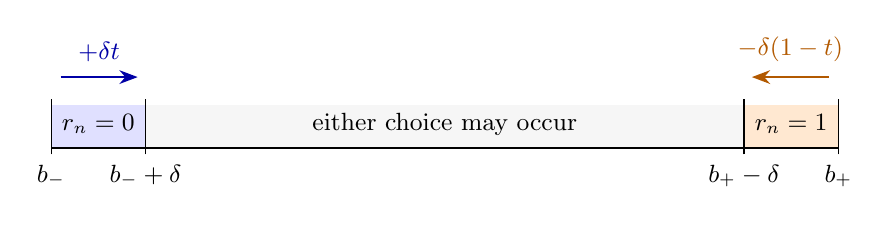
\begin{tikzpicture}[x=1cm,y=1cm,>=Stealth,font=\small]
  \fill[blue!12] (0,0) rectangle (1.2,.55);
  \fill[gray!7] (1.2,0) rectangle (8.8,.55);
  \fill[orange!18] (8.8,0) rectangle (10,.55);
  \draw[thick] (0,0) -- (10,0);
  \foreach \x in {0,1.2,8.8,10} {\draw (\x,-.08) -- (\x,.62);}
  \node[below] at (0,-.09) {$b_-$};
  \node[below] at (1.2,-.09) {$b_-+\delta$};
  \node[below] at (8.8,-.09) {$b_+-\delta$};
  \node[below] at (10,-.09) {$b_+$};
  \node at (.6,.3) {$r_n=0$};
  \node at (9.4,.3) {$r_n=1$};
  \node at (5,.3) {either choice may occur};
  \draw[->,thick,blue!65!black] (.12,.9) -- (1.1,.9);
  \node[above,blue!65!black] at (.61,.97) {$+\delta t$};
  \draw[->,thick,orange!70!black] (9.88,.9) -- (8.9,.9);
  \node[above,orange!70!black] at (9.39,.97) {$-\delta(1-t)$};
\end{tikzpicture}
\caption{The bounded recurrence, schematically. The tested bit forces
an inward step in each endpoint strip; the bit need not be monotone
between them. Each step has length less than $\delta$, so no state
can leave $[b_-,b_+]$. The oracle computation produces the choices
$r_n$, not the numerical states $s_n$.}
\label{fig:bounded-recurrence}
\end{figure}


\medskip
\noindent\emph{Computing the binary choices.}
Let $T$ denote the finite join on the right of
\eqref{eq:four-values}. We show that $(r_n)_{n\ge0}$ is
computable from $T$ by maintaining, relative to $T$, an
oracle-program index $P_n$ satisfying
\[
\Phi_{P_n}^{T}=F(u+s_n).
\]
Initially $P_0$ projects to the first component $F(u)$.
Given $P_n$, read $\Phi_{P_n}^{T}(j)$ and compare it with
the fixed bit $h$ to obtain $r_n$. Select the third component
of $T$ if $r_n=0$ and the fourth if $r_n=1$, namely
\[
F(v-u+\delta(t-r_n)).
\]

Set $a_n=\delta(t-r_n)$. By \eqref{eq:invariant},
$s_n,a_n\in H$ and $|s_n|,|a_n|<\rho$. Equation~\eqref{eq:p}
therefore shows that program $p$, with its two oracle
components simulated by $\Phi_{P_n}^{T}$ and the selected
tuple component, computes
\[
F(v+s_n+a_n)=F(v+s_{n+1}).
\]
Since $|s_{n+1}|<\rho$, Equation~\eqref{eq:q} then shows
that program $q$, with this output and the fixed component
$F(u-v)$ as its two oracles, computes $F(u+s_{n+1})$.
Effective substitution of oracle subroutines produces
the next index $P_{n+1}$.

This is an actual computation relative to the fixed tuple.
The indices are constructed using the already computed
branch bits. Inductively each substituted subroutine is
total on its actual oracle, and both outer programs are
valid reductions at the indicated argument pairs. Every
bit computation has finite nesting depth through earlier
indices and terminates. No bound on its running time is
needed. To compute $r_n$, perform the finite construction
through stage $n$.

The program uses only the fixed integers $p,q,j,h$, the
rational $\delta$, and the four tuple components. It does
not compute the numerical states $s_n$, or use
$t,u,v,\rho,b_-,b_+$ as additional real oracles. The finite
program constants may depend on $t,u,v$, as allowed in the
pointwise reduction \eqref{eq:four-values}.

\medskip
\noindent\emph{Recovering the parameter.}
Summing \eqref{eq:recurrence} gives
\[
s_N=\delta\left(Nt-\sum_{n<N}r_n\right).
\]
Because $|s_N|<\rho<1$, the $T$-computable rational numbers
$A_N=N^{-1}\sum_{n<N}r_n$ satisfy
\begin{equation}\label{eq:error}
|t-A_N|<\frac{1}{N\delta}\qquad(N\ge1).
\end{equation}
For a rational query $a$, search for an $N$ such that
$a<A_N-1/(N\delta)$ or $a>A_N+1/(N\delta)$, and return
the corresponding cut bit. Irrationality of $t$ guarantees
termination. The rational $\delta$ makes the error bound
effective, so this computes $C(t)$ from $T$ and proves
\eqref{eq:four-values}.
\end{proof}

\begin{remark}\label{rem:nonuniform}
The parameter $\delta$ and the reduction program in
Proposition~\ref{prop:recovery} need not be selected
effectively from $(u,v)$. The conclusion is that the
reduction exists for every pair in a comeager set.
The category avoidance argument allows precisely this
form of nonuniformity.
\end{remark}

\section{Rigidity and biinterpretability}
\label{sec:rigidity}

We now apply the recovery construction to the full degree
structure.

\begin{proof}[Proof of Theorem~\ref{thm:rigidity}]
Fix an arbitrary order automorphism $\pi$ and take the
Borel map $F$ given by Lemma~\ref{lem:lift}. Fix an
irrational $t\in(0,1)$. Proposition~\ref{prop:recovery}
gives a comeager set $G_t$ of pairs $(u,v)$ for which
\eqref{eq:four-values} holds with a suitable rational
$\delta\in(0,1)$.

For such a pair, put
$\mathbf b=d(t)\vee d(u)\vee d(v)$.
Each argument in the four values on the right of
\eqref{eq:four-values} is a rational linear combination
of $t,u,v,1$. Lemma~\ref{lem:cuts} bounds its degree by
$\mathbf b$, and Equation~\eqref{eq:representation}
bounds the degree of its $F$-value by $\pi(\mathbf b)$.
The same upper bound holds for the finite join of the
four values. Thus
\[
d(t)\leT \pi\bigl(d(t)\vee d(u)\vee d(v)\bigr)
\qquad((u,v)\in G_t).
\]
Applying the inverse order automorphism yields
\begin{equation}\label{eq:generic-bound}
\pi^{-1}(d(t))\leT d(t)\vee d(u)\vee d(v)
\qquad((u,v)\in G_t).
\end{equation}

Choose one fixed set $Y$ representing $\pi^{-1}(d(t))$.
If $Y\not\leT C(t)$, Lemma~\ref{lem:avoidance} says that
\[
\{(u,v):Y\leT C(t)\oplus C(u)\oplus C(v)\}
\]
is meager. But \eqref{eq:generic-bound} puts the
comeager set $G_t$ inside this set, contradicting the
Baire Category Theorem for $\R^2$. Consequently
\[
\pi^{-1}(d(t))\leT d(t).
\]
The set $Y$ is fixed before the pair varies. No common
index for the reductions in \eqref{eq:generic-bound}
is required.

The irrational $t$ was arbitrary. By Lemma~\ref{lem:cuts},
its degrees cover every noncomputable degree, and the
least degree is fixed. We have therefore proved
\begin{equation}\label{eq:one-sided}
\pi^{-1}(\mathbf a)\leT\mathbf a
\qquad(\mathbf a\in\DT)
\end{equation}
for every order automorphism $\pi$.
Apply this result to the automorphism $\pi^{-1}$ to
obtain $\pi(\mathbf a)\leT\mathbf a$. Applying $\pi$
to \eqref{eq:one-sided} gives
$\mathbf a\leT\pi(\mathbf a)$. Antisymmetry now gives
$\pi(\mathbf a)=\mathbf a$ for every degree.
\end{proof}

The second application uses Theorem~\ref{thm:representation}
for the inverse degree automorphism. It does not require
an inverse of $F$, which may have nontrivial fibers.

\begin{corollary}\label{cor:biinterpretability}
The Turing-degree ordering is biinterpretable without parameters
with full second-order arithmetic, in the sense of
\cite[Definition~7.5.1]{SlamanWoodin2005}.
\end{corollary}

\begin{proof}
Slaman and Woodin prove that this property is equivalent to
rigidity \cite[Theorem~7.5.3]{SlamanWoodin2005}.
Apply Theorem~\ref{thm:rigidity}.
\end{proof}

\begingroup
\small
\begin{thebibliography}{99}

\bibitem{GroszekSlaman1998}
M.~J.~Groszek and T.~A.~Slaman,
A basis theorem for perfect sets,
\emph{Bulletin of Symbolic Logic} \textbf{4} (1998), no.~2,
204--209.
\href{https://doi.org/10.2307/421023}{DOI}.
\href{https://math.berkeley.edu/~slaman/papers/prikry.pdf}{Author's version},
dated 17 November 2000, whose lemma numbering is used here.

\bibitem{JockuschSolovay1977}
C.~G.~Jockusch, Jr., and R.~M.~Solovay,
Fixed points of jump preserving automorphisms of degrees,
\emph{Israel Journal of Mathematics} \textbf{26} (1977), no.~1,
91--94.
\href{https://doi.org/10.1007/BF03007659}{DOI}.

\bibitem{KjosHanssen2018}
B.~Kjos-Hanssen,
Permutations of the integers induce only the trivial automorphism
of the Turing degrees,
\emph{Bulletin of Symbolic Logic} \textbf{24} (2018), no.~2,
165--174.
\href{https://doi.org/10.1017/bsl.2018.15}{DOI}.
\href{https://arxiv.org/abs/1603.00525v1}{arXiv:1603.00525v1}.

\bibitem{KumarShelah2023}
A.~Kumar and S.~Shelah,
Large Turing independent sets,
\emph{Proceedings of the American Mathematical Society}
\textbf{151} (2023), no.~1, 355--367.
\href{https://doi.org/10.1090/proc/16081}{DOI}.

\bibitem{LutzSiskind2025}
P.~Lutz and B.~Siskind,
Part 1 of Martin's conjecture for order-preserving and
measure-preserving functions,
\emph{Journal of the American Mathematical Society}
\textbf{38} (2025), no.~2, 319--367.
\href{https://doi.org/10.1090/jams/1046}{DOI}.
\href{https://arxiv.org/abs/2305.19646v3}{arXiv:2305.19646v3},
whose theorem numbering is used here.

\bibitem{MarkerDST}
D.~Marker,
\href{https://www.math.uic.edu/~marker/math512/dst.pdf}{\emph{Descriptive Set Theory}},
course notes, Fall 2002.

\bibitem{NerodeShore1980}
A.~Nerode and R.~A.~Shore,
Reducibility orderings: theories, definability and automorphisms,
\emph{Annals of Mathematical Logic} \textbf{18} (1980), no.~1,
61--89.
\href{https://doi.org/10.1016/0003-4843(80)90004-2}{DOI}.

\bibitem{Shore2007}
R.~A.~Shore,
Direct and local definitions of the Turing jump,
\emph{Journal of Mathematical Logic} \textbf{7} (2007), no.~2,
229--262.

\bibitem{ShoreSlaman1999}
R.~A.~Shore and T.~A.~Slaman,
Defining the Turing jump,
\emph{Mathematical Research Letters} \textbf{6} (1999), no.~5--6,
711--722.
\href{https://math.berkeley.edu/~slaman/papers/jump.pdf}{Author's version}.

\bibitem{SlamanGlobal}
T.~A.~Slaman,
Global properties of the Turing degrees and the Turing jump,
in \emph{Computational Prospects of Infinity, Part I: Tutorials},
C.~Chong, Q.~Feng, T.~A.~Slaman, W.~H.~Woodin,
and Y.~Yang (eds.),
Lecture Notes Series, Institute for Mathematical Sciences,
National University of Singapore, vol.~14,
World Scientific, Hackensack, NJ, 2008, pp.~83--101.
\href{https://doi.org/10.1142/9789812794055_0002}{DOI}.
\href{https://math.berkeley.edu/~slaman/papers/IMS_slaman.pdf}{Author's version},
whose theorem numbering is used here.

\bibitem{SlamanWoodin2005}
T.~A.~Slaman and W.~H.~Woodin,
\href{https://math.berkeley.edu/~slaman/talks/sw.pdf}{\emph{Definability in Degree Structures}},
unpublished manuscript, 21 July 2005.

\bibitem{Soare1987}
R.~I.~Soare,
\href{https://link.springer.com/book/9783540666813}{\emph{Recursively Enumerable Sets and Degrees:
A Study of Computable Functions and Computably Generated Sets}},
Perspectives in Mathematical Logic,
Springer-Verlag, Berlin, 1987.

\bibitem{Turing1939}
A.~M.~Turing,
Systems of logic based on ordinals,
\emph{Proceedings of the London Mathematical Society}
(2) \textbf{45} (1939), 161--228.
\href{https://doi.org/10.1112/plms/s2-45.1.161}{DOI}.

\end{thebibliography}
\endgroup

\end{document}
